\documentclass[runningheads]{llncs}

\renewcommand{\labelenumii}{\theenumii}
\renewcommand{\theenumii}{\theenumi.\arabic{enumii}.}

\usepackage{graphicx}
\usepackage{hyperref} %might be better to uncomment this
\usepackage{subfig}
\usepackage{algpseudocode}
\usepackage{algorithm}

% Used for displaying a sample figure. If possible, figure files should
% be included in EPS format.
%
% If you use the hyperref package, please uncomment the following line
% to display URLs in blue roman font according to Springer's eBook style:
\renewcommand\UrlFont{\color{blue}\rmfamily}

\begin{document}
%
%\title{Contribution Title\thanks{Supported by organization x.}}
\title{[SCIR] Raport 1}
%
%\titlerunning{very very very }
% If the paper title is too long for the running head, you can set
% an abbreviated paper title here

\author{Bartłomiej Mastej}
%
%
\institute{Warsaw University of Technology, Warsaw, Poland}

%
\maketitle              % typeset the header of the contribution
%
%
%
%
\section{Cel projektu}
Celem projektu jest stworzenie stacji pogodowej, która będzie zbierała dane za pomocą zintegrowanego czujnika wilgotności i temperatury oraz danych z kamerki.
Dane z kamerki mają być wstępnie przetważane lokalnie (Edge computing), a następnie wysyłane do chumury, gdzie na podstawie danych historycznych oraz danych z czujnika wilgotności i temperatury będą analizowane dalej. Ma to na celu przewidywanie temperatury "rzeczywistej" np poprzez wykrywanie opadów/zachmórzenia.

W celu zrealizowani projektu została wybrana platforma Raspberry Pi 4 model B, gdyż zapewnia względnie dużą moc obliczeniową, wystarczającą do prowadzenia prostej analizy danych lokalnie. Ponadto posiada wbudowany moduł wifi, co ułatwia komunikację z chmurą.

Cała dokumentacja do projektu znajduje się na GitHub'ie: \url{https://github.com/bartoszlomiej/weather-forecaster}.

\section{Schemat i części}
\begin{figure}
  %width=\textwidth
  \centering
  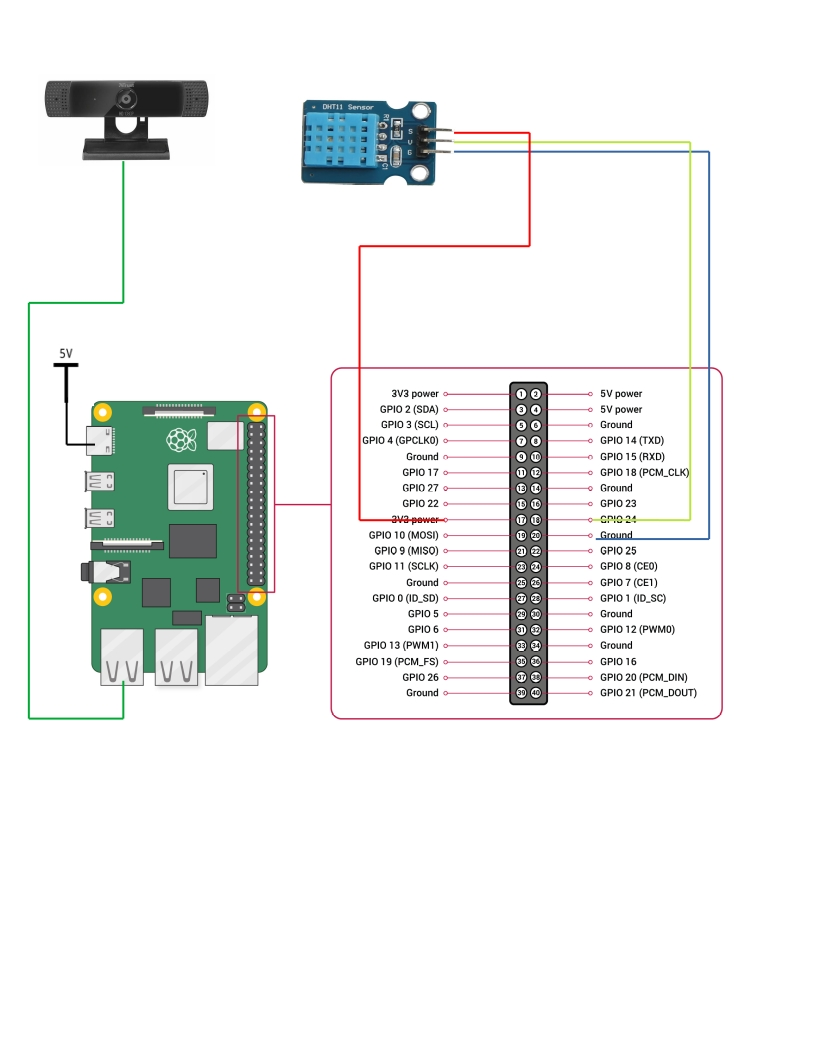
\includegraphics[width=\textwidth]{schemat.jpg}
\caption{Schemat podłączeń czujników do Raspberry Pi} \label{fig1}
\end{figure}
Użyte części:
\begin{enumerate}
\item Raspberry Pi 4 model B - platforma uruchmieniowa czujników oraz węzeł komunikacji,
\item DHT11 - czujnik temperatury i wilgotności,
\item TrustGX1160 - kamerka
\end{enumerate}

\section{Zbieranie danych z czujników}
\subsection{Konfiguracja Raspberry Pi}
Jako, że na Rasberry Pi został wgrany system operacyjny, komunikacja odbywa się po SSH. W celu skonfigurowania SSH należało dodać sieć wifi przy instalacji oraz dodać pusty plik $.ssh$ w folderze $/boot$ urządzenia. Pliki są wysyłane z komputera do Raspberry poprzez scp (secure copy, działające na zasadzie ssh). Potrzebne biblioteki zostały pobrane poprzez narzędzie $PIP$ języka $Python$.
\subsection{Czujnik wilgotności i temperatury - DHT11}
Czujnik DHT11 jest cyfrowy. W celu zbierania danych została wykorzystane biblioteki do Python'a: $RPI$ oraz $dht11$. Pierwsza z nich odpowiada za wykorzystanie Pinów ogólnego użytku (GPIO - general purpuse input output) i została wykorzsytana do pobierania danych z czujnika na pin'ie nr. 24. Natomiast druga biblioteka umożliwia wykorzystanie wcześniej wybranego pin'u do obioru danych z czujnika.
\subsection{Kamerka TrustGX1160}
Do zczytywania danych z kamerki została wykorzystana biblioteka $OpenCV$. Za pomocą funkcji $VideoCapture(0)$ kamerka jest uruchomiana, następnie wykonywane jest zdjęcie za pomocą funkcji $read()$. Następnie zdjęcie zapisywane jest do pliku.

\end{document}
